\documentclass{report}
\usepackage{tikz}
\usepackage{subcaption}

\begin{document}
\begin{figure}
  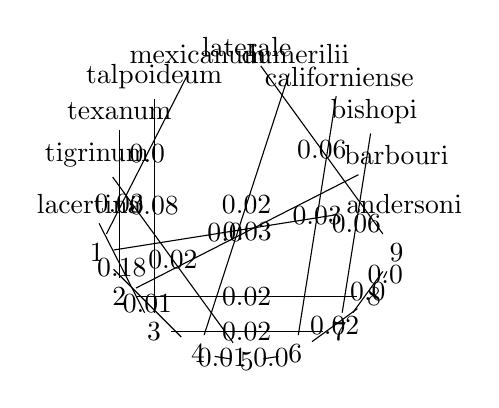
\begin{tikzpicture}
      \draw
        (0.0:2) node (andersoni){andersoni}
        (18.0:2) node (barbouri){barbouri}
        (36.0:2) node (bishopi){bishopi}
        (54.0:2) node (californiense){californiense}
        (72.0:2) node (dumerilii){dumerilii}
        (90.0:2) node (laterale){laterale}
        (108.0:2) node (mexicanum){mexicanum}
        (126.0:2) node (talpoideum){talpoideum}
        (144.0:2) node (texanum){texanum}
        (162.0:2) node (tigrinum){tigrinum}
        (180.0:2) node (lacertina){lacertina}
        (198.0:2) node (1){1}
        (216.0:2) node (2){2}
        (234.0:2) node (3){3}
        (252.0:2) node (4){4}
        (270.0:2) node (5){5}
        (288.0:2) node (6){6}
        (306.0:2) node (7){7}
        (324.0:2) node (8){8}
        (342.0:2) node (9){9};
      \begin{scope}[-]
        \draw (andersoni) to node[] {0.0} (1);
        \draw (barbouri) to node[] {0.03} (2);
        \draw (bishopi) to node[] {0.06} (7);
        \draw (californiense) to node[] {0.03} (6);
        \draw (dumerilii) to node[] {0.02} (4);
        \draw (laterale) to node[] {0.06} (9);
        \draw (mexicanum) to node[] {0.0} (1);
        \draw (talpoideum) to node[] {0.08} (3);
        \draw (texanum) to node[] {0.03} (2);
        \draw (tigrinum) to node[] {0.02} (5);
        \draw (lacertina) to node[] {0.18} (3);
        \draw (1) to node[] {0.01} (4);
        \draw (2) to node[] {0.02} (8);
        \draw (3) to node[] {0.02} (7);
        \draw (4) to node[] {0.01} (5);
        \draw (5) to node[] {0.0} (6);
        \draw (6) to node[] {0.02} (8);
        \draw (7) to node[] {0.0} (9);
        \draw (8) to node[] {0.0} (9);
      \end{scope}
    \end{tikzpicture}
  \caption{{nombre}}
\end{figure}
\end{document}